\documentclass{extbook}[14pt]
\usepackage{multicol, enumerate, enumitem, hyperref, color, soul, setspace, parskip, fancyhdr, amssymb, amsthm, amsmath, bbm, latexsym, units, mathtools}
\everymath{\displaystyle}
\usepackage[headsep=0.5cm,headheight=0cm, left=1 in,right= 1 in,top= 1 in,bottom= 1 in]{geometry}
\usepackage{dashrule}  % Package to use the command below to create lines between items
\newcommand{\litem}[1]{\item #1

\rule{\textwidth}{0.4pt}}
\pagestyle{fancy}
\lhead{}
\chead{Answer Key for Makeup Progress Quiz 1 Version A}
\rhead{}
\lfoot{6018-3080}
\cfoot{}
\rfoot{Spring 2021}
\begin{document}
\textbf{This key should allow you to understand why you choose the option you did (beyond just getting a question right or wrong). \href{https://xronos.clas.ufl.edu/mac1105spring2020/courseDescriptionAndMisc/Exams/LearningFromResults}{More instructions on how to use this key can be found here}.}

\textbf{If you have a suggestion to make the keys better, \href{https://forms.gle/CZkbZmPbC9XALEE88}{please fill out the short survey here}.}

\textit{Note: This key is auto-generated and may contain issues and/or errors. The keys are reviewed after each exam to ensure grading is done accurately. If there are issues (like duplicate options), they are noted in the offline gradebook. The keys are a work-in-progress to give students as many resources to improve as possible.}

\rule{\textwidth}{0.4pt}

\begin{enumerate}\litem{
Construct the lowest-degree polynomial given the zeros below. Then, choose the intervals that contain the coefficients of the polynomial in the form $ax^3+bx^2+cx+d$.
\[ -3, \frac{-3}{4}, \text{ and } \frac{7}{3} \]The solution is \( 12x^{3} +17 x^{2} -78 x -63 \), which is option D.\begin{enumerate}[label=\Alph*.]
\item \( a \in [12, 13], b \in [14, 21], c \in [-78, -75], \text{ and } d \in [61, 66] \)

$12x^{3} +17 x^{2} -78 x + 63$, which corresponds to multiplying everything correctly except the constant term.
\item \( a \in [12, 13], b \in [-57, -54], c \in [22, 39], \text{ and } d \in [61, 66] \)

$12x^{3} -55 x^{2} +36 x + 63$, which corresponds to multiplying out $(x -3)(4x + 3)(3x -7)$.
\item \( a \in [12, 13], b \in [-23, -13], c \in [-78, -75], \text{ and } d \in [61, 66] \)

$12x^{3} -17 x^{2} -78 x + 63$, which corresponds to multiplying out $(x -3)(4x -3)(3x + 7)$.
\item \( a \in [12, 13], b \in [14, 21], c \in [-78, -75], \text{ and } d \in [-63, -57] \)

* $12x^{3} +17 x^{2} -78 x -63$, which is the correct option.
\item \( a \in [12, 13], b \in [-78, -63], c \in [131, 136], \text{ and } d \in [-63, -57] \)

$12x^{3} -73 x^{2} +132 x -63$, which corresponds to multiplying out $(x -3)(4x -3)(3x -7)$.
\end{enumerate}

\textbf{General Comment:} To construct the lowest-degree polynomial, you want to multiply out $(x + 3)(4x + 3)(3x -7)$
}
\litem{
Describe the end behavior of the polynomial below.
\[ f(x) = 3(x - 9)^{5}(x + 9)^{6}(x - 3)^{3}(x + 3)^{4} \]The solution is the graph below, which is option C.
\begin{center}
    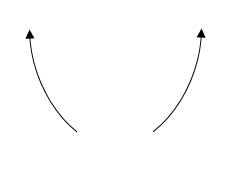
\includegraphics[width=0.3\textwidth]{../Figures/polyEndBehaviorCA.png}
\end{center}\begin{enumerate}[label=\Alph*.]
\begin{multicols}{2}
\item 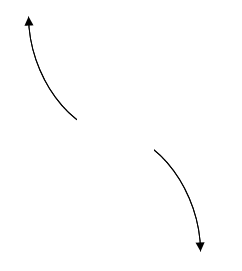
\includegraphics[width = 0.3\textwidth]{../Figures/polyEndBehaviorAA.png}
\item 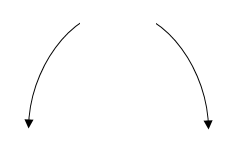
\includegraphics[width = 0.3\textwidth]{../Figures/polyEndBehaviorBA.png}
\item 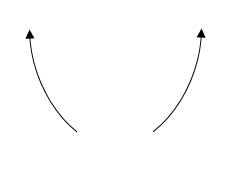
\includegraphics[width = 0.3\textwidth]{../Figures/polyEndBehaviorCA.png}
\item 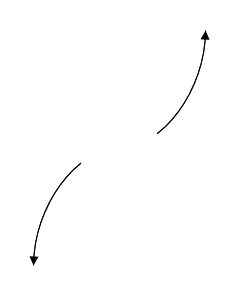
\includegraphics[width = 0.3\textwidth]{../Figures/polyEndBehaviorDA.png}
\end{multicols}\item None of the above.\end{enumerate}
\textbf{General Comment:} Remember that end behavior is determined by the leading coefficient AND whether the \textbf{sum} of the multiplicities is positive or negative.
}
\litem{
Construct the lowest-degree polynomial given the zeros below. Then, choose the intervals that contain the coefficients of the polynomial in the form $x^3+bx^2+cx+d$.
\[ -2 - 4 i \text{ and } 2 \]The solution is \( x^{3} +2 x^{2} +12 x -40 \), which is option D.\begin{enumerate}[label=\Alph*.]
\item \( b \in [0.5, 1.3], c \in [-0.75, 0.06], \text{ and } d \in [-6.3, -3.5] \)

$x^{3} + x^{2} -4$, which corresponds to multiplying out $(x + 2)(x -2)$.
\item \( b \in [0.5, 1.3], c \in [1.85, 3.06], \text{ and } d \in [-10.4, -7.1] \)

$x^{3} + x^{2} +2 x -8$, which corresponds to multiplying out $(x + 4)(x -2)$.
\item \( b \in [-2.2, 0.7], c \in [11.7, 12.65], \text{ and } d \in [39.5, 42.6] \)

$x^{3} -2 x^{2} +12 x + 40$, which corresponds to multiplying out $(x-(-2 - 4 i))(x-(-2 + 4 i))(x + 2)$.
\item \( b \in [1.5, 2.9], c \in [11.7, 12.65], \text{ and } d \in [-41.8, -38.7] \)

* $x^{3} +2 x^{2} +12 x -40$, which is the correct option.
\item \( \text{None of the above.} \)

This corresponds to making an unanticipated error or not understanding how to use nonreal complex numbers to create the lowest-degree polynomial. If you chose this and are not sure what you did wrong, please contact the coordinator for help.
\end{enumerate}

\textbf{General Comment:} Remember that the conjugate of $a+bi$ is $a-bi$. Since these zeros always come in pairs, we need to multiply out $(x-(-2 - 4 i))(x-(-2 + 4 i))(x-(2))$.
}
\litem{
Construct the lowest-degree polynomial given the zeros below. Then, choose the intervals that contain the coefficients of the polynomial in the form $ax^3+bx^2+cx+d$.
\[ \frac{7}{3}, \frac{-1}{4}, \text{ and } \frac{6}{5} \]The solution is \( 60x^{3} -197 x^{2} +115 x + 42 \), which is option D.\begin{enumerate}[label=\Alph*.]
\item \( a \in [57, 65], b \in [73, 89], c \in [-153, -150], \text{ and } d \in [-43, -39] \)

$60x^{3} +83 x^{2} -151 x -42$, which corresponds to multiplying out $(3x + 7)(4x + 1)(5x -6)$.
\item \( a \in [57, 65], b \in [-199, -195], c \in [108, 120], \text{ and } d \in [-43, -39] \)

$60x^{3} -197 x^{2} +115 x -42$, which corresponds to multiplying everything correctly except the constant term.
\item \( a \in [57, 65], b \in [196, 200], c \in [108, 120], \text{ and } d \in [-43, -39] \)

$60x^{3} +197 x^{2} +115 x -42$, which corresponds to multiplying out $(3x + 7)(4x -1)(5x + 6)$.
\item \( a \in [57, 65], b \in [-199, -195], c \in [108, 120], \text{ and } d \in [33, 43] \)

* $60x^{3} -197 x^{2} +115 x + 42$, which is the correct option.
\item \( a \in [57, 65], b \in [47, 60], c \in [-185, -182], \text{ and } d \in [33, 43] \)

$60x^{3} +53 x^{2} -185 x + 42$, which corresponds to multiplying out $(3x + 7)(4x -1)(5x -6)$.
\end{enumerate}

\textbf{General Comment:} To construct the lowest-degree polynomial, you want to multiply out $(3x -7)(4x + 1)(5x -6)$
}
\litem{
Construct the lowest-degree polynomial given the zeros below. Then, choose the intervals that contain the coefficients of the polynomial in the form $x^3+bx^2+cx+d$.
\[ 5 - 4 i \text{ and } -1 \]The solution is \( x^{3} -9 x^{2} +31 x + 41 \), which is option B.\begin{enumerate}[label=\Alph*.]
\item \( b \in [-7, 7], c \in [-10, 4], \text{ and } d \in [-13, -4] \)

$x^{3} + x^{2} -4 x -5$, which corresponds to multiplying out $(x -5)(x + 1)$.
\item \( b \in [-9, -4], c \in [29, 36], \text{ and } d \in [37, 44] \)

* $x^{3} -9 x^{2} +31 x + 41$, which is the correct option.
\item \( b \in [4, 12], c \in [29, 36], \text{ and } d \in [-43, -39] \)

$x^{3} +9 x^{2} +31 x -41$, which corresponds to multiplying out $(x-(5 - 4 i))(x-(5 + 4 i))(x -1)$.
\item \( b \in [-7, 7], c \in [3, 13], \text{ and } d \in [0, 8] \)

$x^{3} + x^{2} +5 x + 4$, which corresponds to multiplying out $(x + 4)(x + 1)$.
\item \( \text{None of the above.} \)

This corresponds to making an unanticipated error or not understanding how to use nonreal complex numbers to create the lowest-degree polynomial. If you chose this and are not sure what you did wrong, please contact the coordinator for help.
\end{enumerate}

\textbf{General Comment:} Remember that the conjugate of $a+bi$ is $a-bi$. Since these zeros always come in pairs, we need to multiply out $(x-(5 - 4 i))(x-(5 + 4 i))(x-(-1))$.
}
\litem{
Which of the following equations \textit{could} be of the graph presented below?

\begin{center}
    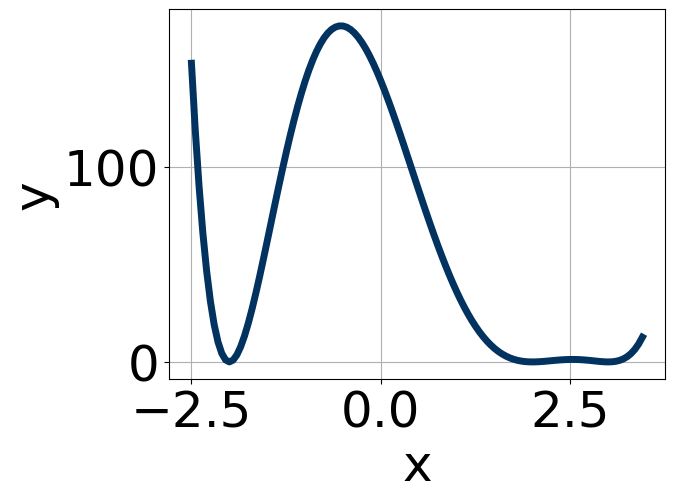
\includegraphics[width=0.5\textwidth]{../Figures/polyGraphToFunctionA.png}
\end{center}


The solution is \( 16(x - 2)^{4} (x + 2)^{4} (x - 3)^{8} \), which is option D.\begin{enumerate}[label=\Alph*.]
\item \( 5(x - 2)^{6} (x + 2)^{11} (x - 3)^{7} \)

The factors $(x + 2)$ and $(x - 3)$ should both have even powers.
\item \( 17(x - 2)^{6} (x + 2)^{10} (x - 3)^{7} \)

The factor $(x - 3)$ should have an even power.
\item \( -5(x - 2)^{4} (x + 2)^{10} (x - 3)^{4} \)

This corresponds to the leading coefficient being the opposite value than it should be.
\item \( 16(x - 2)^{4} (x + 2)^{4} (x - 3)^{8} \)

* This is the correct option.
\item \( -18(x - 2)^{8} (x + 2)^{4} (x - 3)^{7} \)

The factor $(x - 3)$ should have an even power and the leading coefficient should be the opposite sign.
\end{enumerate}

\textbf{General Comment:} General Comments: Draw the x-axis to determine which zeros are touching (and so have even multiplicity) or cross (and have odd multiplicity).
}
\litem{
Describe the zero behavior of the zero $x = -3$ of the polynomial below.
\[ f(x) = -2(x - 3)^{2}(x + 3)^{3}(x - 4)^{4}(x + 4)^{7} \]The solution is the graph below, which is option A.
\begin{center}
    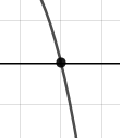
\includegraphics[width=0.3\textwidth]{../Figures/polyZeroBehaviorCopyAA.png}
\end{center}\begin{enumerate}[label=\Alph*.]
\begin{multicols}{2}
\item 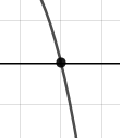
\includegraphics[width = 0.3\textwidth]{../Figures/polyZeroBehaviorCopyAA.png}
\item 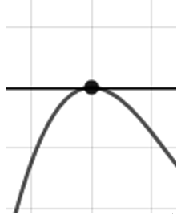
\includegraphics[width = 0.3\textwidth]{../Figures/polyZeroBehaviorCopyBA.png}
\item 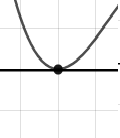
\includegraphics[width = 0.3\textwidth]{../Figures/polyZeroBehaviorCopyCA.png}
\item 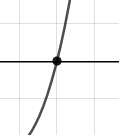
\includegraphics[width = 0.3\textwidth]{../Figures/polyZeroBehaviorCopyDA.png}
\end{multicols}\item None of the above.\end{enumerate}
\textbf{General Comment:} You will need to sketch the entire graph, then zoom in on the zero the question asks about.
}
\litem{
Describe the end behavior of the polynomial below.
\[ f(x) = 9(x - 7)^{4}(x + 7)^{5}(x + 6)^{3}(x - 6)^{4} \]The solution is the graph below, which is option C.
\begin{center}
    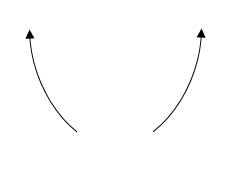
\includegraphics[width=0.3\textwidth]{../Figures/polyEndBehaviorCopyCA.png}
\end{center}\begin{enumerate}[label=\Alph*.]
\begin{multicols}{2}
\item 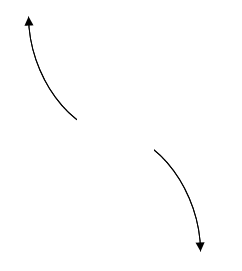
\includegraphics[width = 0.3\textwidth]{../Figures/polyEndBehaviorCopyAA.png}
\item 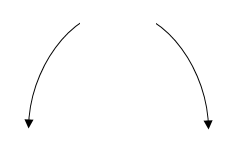
\includegraphics[width = 0.3\textwidth]{../Figures/polyEndBehaviorCopyBA.png}
\item 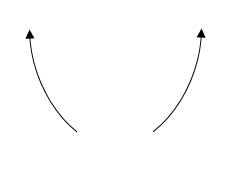
\includegraphics[width = 0.3\textwidth]{../Figures/polyEndBehaviorCopyCA.png}
\item 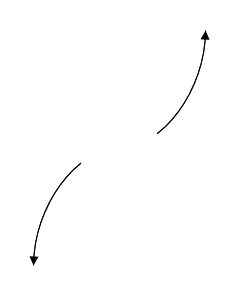
\includegraphics[width = 0.3\textwidth]{../Figures/polyEndBehaviorCopyDA.png}
\end{multicols}\item None of the above.\end{enumerate}
\textbf{General Comment:} Remember that end behavior is determined by the leading coefficient AND whether the \textbf{sum} of the multiplicities is positive or negative.
}
\litem{
Which of the following equations \textit{could} be of the graph presented below?

\begin{center}
    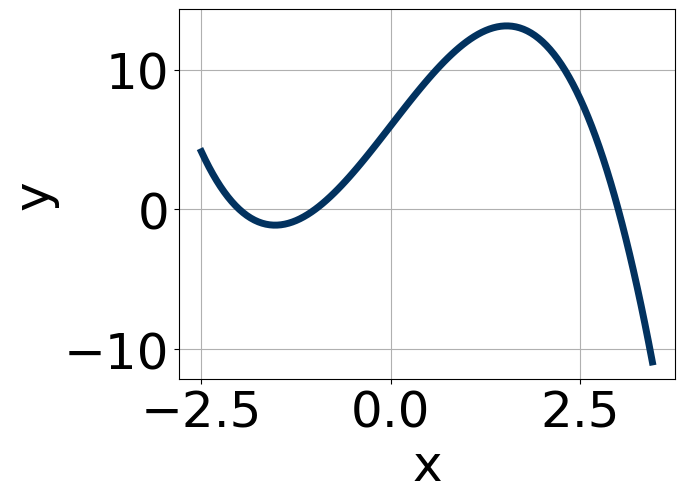
\includegraphics[width=0.5\textwidth]{../Figures/polyGraphToFunctionCopyA.png}
\end{center}


The solution is \( -12(x + 2)^{11} (x + 1)^{5} (x - 3)^{9} \), which is option D.\begin{enumerate}[label=\Alph*.]
\item \( -3(x + 2)^{10} (x + 1)^{10} (x - 3)^{9} \)

The factors $-2$ and $-1$ have have been odd power.
\item \( 20(x + 2)^{7} (x + 1)^{11} (x - 3)^{7} \)

This corresponds to the leading coefficient being the opposite value than it should be.
\item \( -2(x + 2)^{8} (x + 1)^{9} (x - 3)^{7} \)

The factor $-2$ should have been an odd power.
\item \( -12(x + 2)^{11} (x + 1)^{5} (x - 3)^{9} \)

* This is the correct option.
\item \( 10(x + 2)^{6} (x + 1)^{7} (x - 3)^{11} \)

The factor $(x + 2)$ should have an odd power and the leading coefficient should be the opposite sign.
\end{enumerate}

\textbf{General Comment:} General Comments: Draw the x-axis to determine which zeros are touching (and so have even multiplicity) or cross (and have odd multiplicity).
}
\litem{
Describe the zero behavior of the zero $x = -3$ of the polynomial below.
\[ f(x) = 3(x - 3)^{4}(x + 3)^{5}(x - 9)^{8}(x + 9)^{10} \]The solution is the graph below, which is option D.
\begin{center}
    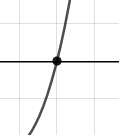
\includegraphics[width=0.3\textwidth]{../Figures/polyZeroBehaviorDA.png}
\end{center}\begin{enumerate}[label=\Alph*.]
\begin{multicols}{2}
\item 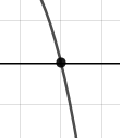
\includegraphics[width = 0.3\textwidth]{../Figures/polyZeroBehaviorAA.png}
\item 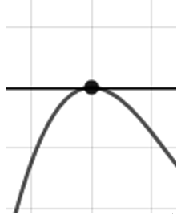
\includegraphics[width = 0.3\textwidth]{../Figures/polyZeroBehaviorBA.png}
\item 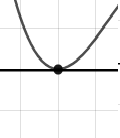
\includegraphics[width = 0.3\textwidth]{../Figures/polyZeroBehaviorCA.png}
\item 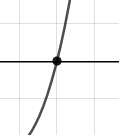
\includegraphics[width = 0.3\textwidth]{../Figures/polyZeroBehaviorDA.png}
\end{multicols}\item None of the above.\end{enumerate}
\textbf{General Comment:} You will need to sketch the entire graph, then zoom in on the zero the question asks about.
}
\end{enumerate}

\end{document}